\documentclass[12pt, a4paper]{article}
\usepackage[utf8]{inputenc}
\usepackage[T1]{fontenc}
\usepackage{hyperref}
\usepackage{fancyvrb}


\usepackage{tikz}
\usepackage{amsmath}
\usetikzlibrary[topaths]


\usetikzlibrary{automata}

\usetikzlibrary{graphs}

\newcount\mycount



\begin{document}

\section*{Rød-svarte trær}

\tikzset{
	treenode/.style = {align=center, inner sep=0pt},
	% Sorte noder
  	node_black/.style = {treenode, circle, white, font=\bfseries, draw=black,fill=black, text width=0.8cm},
	% Røde noder
  	node_red/.style = {treenode, circle, red, draw=red, text width=0.8cm, very thick},
	% Null-pekere
  	node_null/.style = {treenode, rectangle, draw=black, minimum width=0.3cm, minimum height=0.3cm}
}
\begin{center}
% Skal tegne med piler (->), og setter level/.style={opt.} %
\begin{tikzpicture}[->,level/.style={sibling distance = 2cm, level distance = 1.5cm}] 
\node [node_black] {38}
    	child{ node [node_red] {19} 
		child{node [node_black] {12}
			child{node [node_red] {8}}
			child{node [node_null] {}}
		}
		child{node [node_black] {31}}
	}
    	child{ node [node_black] {41} }
; 
\end{tikzpicture}
\end{center}

Å tegne trær på denne måten krever ingen tilleggsbiblioteker fra TikZ. Dette er et eksempel på tegning med \textit{parametre}. Utseende til nodene i treet er definert som parametre som har et sett med \texttt{.style}-opsjoner.
\begin{Verbatim}[fontsize=\small, frame=single]
\tikzset{
   treenode/.style = {align=center, inner sep=0pt},
	
   % Sorte noder
   node_black/.style = {treenode, circle, white, 
			font=\bfseries, draw=black,
			fill=black, text width=0.8cm},
   % Røde noder
   node_red/.style = {treenode, circle, red, draw=red, 
	              text width=0.8cm, very thick},
   % Null-pekere
   node_null/.style = {treenode, rectangle, draw=black, 
		       minimum width=0.3cm, minimum height=0.3cm}
}
\end{Verbatim}
Starter med å definere \texttt{treenode}, som er felles for alle typer noder. Røde og sorte noder tegnes som \texttt{circle}, hvor sorte noder har \texttt{fill=black} og tekstfarge \texttt{white}, mens røde noder har rødt omriss med \texttt{draw=red}, og tekstfarge \texttt{red}. Null-nodene sier vi skal være sorte \texttt{rectangle}. Tegnes som små kvadrater på 0.3 cm $\times$ 0.3 cm.

\newpage
\subsection*{Bygge et tre}
\begin{Verbatim}[fontsize=\small, frame=single]
\begin{tikzpicture}[->,level/.style={ sibling distance = 2cm, 
                    level distance = 1.5cm }] 
\node [node_black] {38}
    child {node [node_red] {19} 
        child {node [node_black] {12}
             child {node [node_red] {8} }
             child {node [node_null] {} }
        }
        child {node [node_black] {31} }
    }
    child { node [node_black] {41} }
; 
\end{tikzpicture}
\end{Verbatim}

Setter forskjellige opsjoner med:
\begin{center}
\texttt{\{tikzpicture\}[->, level/.style=\{sibling distance=2cm, level distance)=1.5cm\}]}
\end{center}
Her sier vi at treet skal tegnes med piler (\texttt{->}), og at stilen (\texttt{.style}) for distansen mellom søskennoder skal være 2 cm, og distansen mellom barn og foreldre skal være 1.5 cm.

Videre så tegnes treet ved å definere roten:
\begin{center}
\texttt{\textbackslash node [opt.] \{node value\} ;} 
\end{center}
Så kan man bygge treet ved å legge inn barna til roten, osv.:
\vspace{1em}

\texttt{\textbackslash node [opt.] \{node value\} \\
\indent \indent child \{node [opt.] \{node value\} \} ;} 


\newpage
\subsection*{Eksempel med flere lag}
Her er et eksempel på et tre hvor første, andre, og tredje lag med noder har forskjellige distanser mellom søskennoder.

\begin{center}
\begin{tikzpicture}[every node/.style={},level 2/.style={sibling distance=20mm},level 3/.style={sibling distance=10mm}, level distance=30pt]
\node {S}
	child { node{A} 
		child { node {A} 
			child { node {(} }
			child { node {)} }
		}
		child { node {A} 
			child { node {(} }
			child { node {A} 
				child { node {(} }
				child { node {)} }
			}
			child { node {)} }
		}
	};
\end{tikzpicture}
\end{center}

\begin{Verbatim}[fontsize=\small, frame=single]
\begin{tikzpicture}[every node/.style={},
                    level 2/.style={sibling distance=20mm},
                    level 3/.style={sibling distance=10mm}, 
                    level distance=30pt]
\node {S}
    child { node{A} 
        child { node {A} 
            child { node {(} }
            child { node {)} }
        }
        child { node {A} 
            child { node {(} }
            child { node {A} 
                child { node {(} }
                child { node {)} }
            }
            child { node {)} }
        }
    }
;
\end{tikzpicture}
\end{Verbatim}

\newpage

%%% GRAFER %%%
\section*{Grafer}

\begin{center}
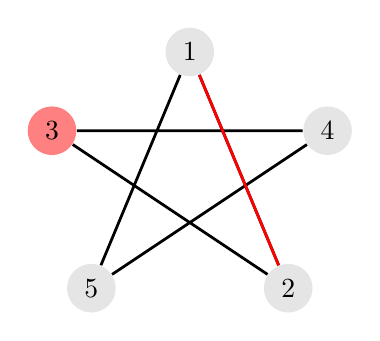
\begin{tikzpicture}[scale=5]
	 \tikzstyle{vertex}=[circle,fill=black!10]
	 \tikzstyle{selected vertex} = [vertex, fill=red!50]

	 \tikzstyle{selected edge} = [draw,line width=1pt,-,red!100]
	 \tikzstyle{edge} = [-,black,line width=1pt]

	 \node[vertex] (v1) at (1.25,1.7) 				{1};
	 \node[vertex] (v2) at (1.5,1.1) 					{2};
	 \node[selected vertex] (v3) at (0.9,1.5) 		{3};
	 \node[vertex] (v4) at (1.6,1.5) 					{4};
	 \node[vertex] (v5) at (1,1.1) 					{5};

	\draw[edge] (v1)  -- (v2) -- (v3) -- (v4) -- (v5) -- (v1); 
	\draw[selected edge] (v1) -- (v2);
\end{tikzpicture}
\end{center}

Det fins enklere måter å tegne grafer på enn dette, men jeg syns denne måten er fin. Den krever heller ingen andre biblioteker eller pakker enn TikZ selv. Eksempel på en veldig mye enklere måte kommer på slutten av denne seksjonen.

Vi starter med å definere de forskjellige elementene til en graf.

\begin{Verbatim}[fontsize=\small, frame=single]
\begin{tikzpicture}
    \tikzstyle{vertex} = [circle,fill=black!10]
    \tikzstyle{selected vertex} = [vertex, fill=red!50]

    \tikzstyle{selected edge} = [draw,line width=1pt,-,red!100]
    \tikzstyle{edge} = [-,black,line width=1pt]
\end{tikzpicture}
\end{Verbatim}
Her fortelle vi at \texttt{vertex}er (eller noder), skal være sirkler som er fylt med sort med en gjennomsiktighet på 10\%. Markerte noder skal også være fylt, da med en annen farge.
\begin{center}

\begin{tikzpicture}[scale=2]
	 \tikzstyle{vertex}=[circle,fill=black!10]
	 \tikzstyle{selected vertex} = [vertex, fill=red!50]

	 \node[vertex] (v1) at (1,1) 				{x};
	 \node[selected vertex] (v2) at (2,1) 		{y};
\end{tikzpicture}
\end{center}

\noindent Kanter skal tegnes som sorte linjer (\texttt{[-, black $\dots$]}). Og markerte kanter skal være røde.

\begin{center}
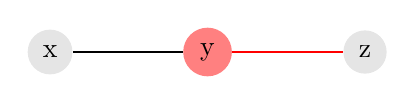
\begin{tikzpicture}[scale=2]
	 \tikzstyle{vertex}=[circle,fill=black!10]
	 \tikzstyle{selected vertex} = [vertex, fill=red!50]
	 \tikzstyle{selected edge} = [draw,line width=1pt,-,red!100]
	 \tikzstyle{edge} = [-,black,line width=1pt]

	 \node[vertex] (v1) at (1,1) 				{x};
	 \node[selected vertex] (v2) at (2,1) 		{y};
	\node[vertex] (v3) at (3,1)					{z};
	\draw[edge] (v1) -- (v2);
	\draw[selected edge] (v2) -- (v3);
\end{tikzpicture}
\end{center}

\newpage
\subsection*{Tegne grafen} For å plassere nodene rundt om på arket sier man hvor man vil de skal være. For eksempelet på toppen (grafen som har stjerne-form), er TikZ-koden som følger:

\begin{Verbatim}[fontsize=\small, frame=single]
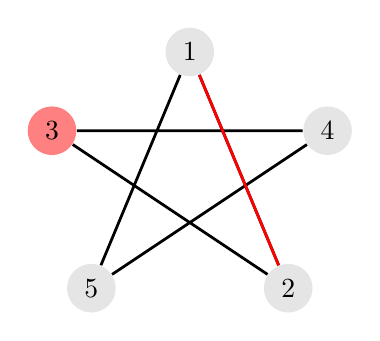
\begin{tikzpicture}[scale=5]
    \tikzstyle{vertex}          = [circle,fill=black!10]
    \tikzstyle{selected vertex} = [vertex, fill=red!50]

    \tikzstyle{selected edge}   = [draw,line width=1pt,-,red!100]
    \tikzstyle{edge}            = [-,black,line width=1pt]

    \node[vertex]          (v1) at (1.25,1.7) {1};
    \node[vertex]          (v2) at (1.5,1.1)  {2};
    \node[selected vertex] (v3) at (0.9,1.5)  {3};
    \node[vertex]          (v4) at (1.6,1.5)  {4};
    \node[vertex]          (v5) at (1,1.1)    {5};

    \draw[edge]          (v1)--(v2)--(v3)--(v4)--(v5)--(v1); 
    \draw[selected edge] (v1)--(v2);
\end{tikzpicture}
\end{Verbatim}

\newpage

%%% AUTOMATER %%%
\section*{Automater}

\begin{center}

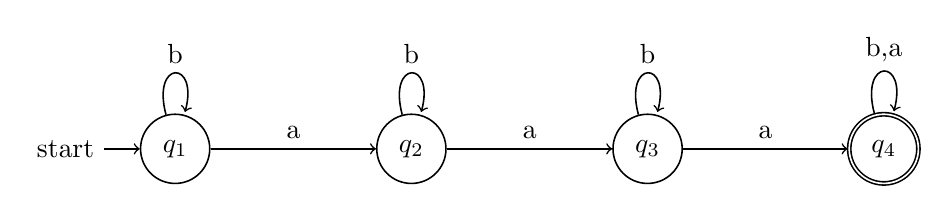
\begin{tikzpicture}[->,auto,node distance=3cm,line width=0.2mm]
  \node[initial,state] 			(A)		 	         {$q_1$};
  \node[state]         			(B) [right of=A] 	{$q_2$};
  \node[state]				(C) [right of=B] 	{$q_3$};
  \node[state,accepting]		(D) [right of=C] 	{$q_4$};

  \path 	(A) edge [loop above] node 			{b} 		(A)
			edge node 						{a} 		(B)
        		(B) edge [loop above] node 			{b} 		(B)
			edge node 						{a} 		(C)
		(C) edge [loop above] node 			{b}		(C)
			edge node 						{a} 		(D)
		(D) edge [loop above] node 			{b,a}	(D);
\end{tikzpicture}
\end{center}

\begin{Verbatim}[fontsize=\small, frame=single]
\begin{tikzpicture}[->,auto,node distance=3cm,line width=0.2mm]
  \node[initial,state   (A) 		{$q_1$};
  \node[state]          (B) [right of=A]    {$q_2$};
  \node[state]	  (C) [right of=B]    {$q_3$};
  \node[state,accepting](D) [right of=C]    {$q_4$};

  \path (A) edge [loop above] node 	 {b}   (A)
	    edge node      		 {a}   (B)
        (B) edge [loop above] node 	 {b}   (B)
	    edge node   	  	  {a}   (C)
        (C) edge [loop above] node	  {b}   (C)
	    edge node 	    	  {a}   (D)
        (D) edge [loop above] node 	 {b,a} (D);
\end{tikzpicture}
\end{Verbatim}


For denne måten å tegne automater på, så settes alle parametre som beskriver automaten i definisjonen til \texttt{tikzpicture}. Man må også inkludere \texttt{\textbackslash usetikzlibrary\{automata\}}.
Her har automaten følgende egenskaper:
\begin{center}
\texttt{\{tikzpicture\}[->, auto, node distance=3cm, line width=0.2mm]}
\end{center}
Dette forteller oss at automaten skal tegnes med piler (\texttt{->}), nodene skal ha avstand på 3 cm, og linjene en tykkelse på 0,2 mm. Auto stiller teksten \textit{over} linjene, i stedet for \textit{på} linjene.

\subsection*{Automatens tilstander} En automat har tre typer tilstander: starttilstanden, vanlig tilstand(er), og akepterende tilstand(er).
\begin{center}
\texttt{\textbackslash node[state] (node-name) \{name of state\};}
\end{center}
I tillegg til \texttt{[state]}, så kan man ha med opsjonen \texttt{[initial, state]} for starttilstanden, eller \texttt{[state, accepting]} for aksepterende tilstand.

\subsection*{Stien gjennom automaten}
Stien tegnes gjennom en \texttt{path}. Denne konstrueres på følgende vis:
\begin{center}
\texttt{\textbackslash path (from-node) edge [opt.] node \{weight\} (to-node)}.
\end{center}
Her kan \texttt{[opt]} være \texttt{loop above/below}, \texttt{bend left/right}.

\subsection*{Flittig bever}
Her er en flittig 4-bever. Denne automaten dekker de fleste opsjoner.
\begin{center}
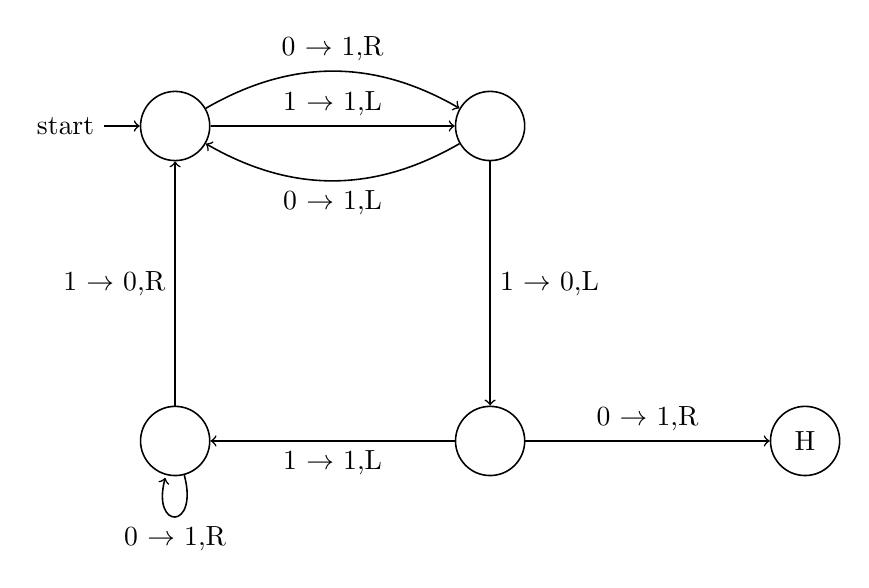
\begin{tikzpicture}[->,auto,node distance=4cm,line width=0.2mm]
  \node[initial,state] 		(A)            			{};
  \node[state] 			(B) [below of=A]   	{};
  \node[state] 			(C) [right of=A]    		{};
  \node[state] 			(D) [below of=C] 		{};
  \node[state]         		(E) [right of=D] 		{H};

  \path 	(A) edge node 				{1 $\rightarrow$ 1,L} 		(C)
		(A) edge [bend left] node 		{0 $\rightarrow$ 1,R} 		(C)
		(C) edge [bend left] node 		{0 $\rightarrow$ 1,L} 		(A)
		(B) edge node 				{1 $\rightarrow$ 0,R} 		(A)
		(B) edge [loop below] node 	{0 $\rightarrow$ 1,R} 		(B)
		(D) edge node 				{1 $\rightarrow$ 1,L} 		(B)
		(C) edge node 				{1 $\rightarrow$ 0,L} 		(D)
		(D) edge node		 		{0 $\rightarrow$ 1,R} 		(E);
\end{tikzpicture}
\end{center}

\begin{Verbatim}[fontsize=\small, frame=single]
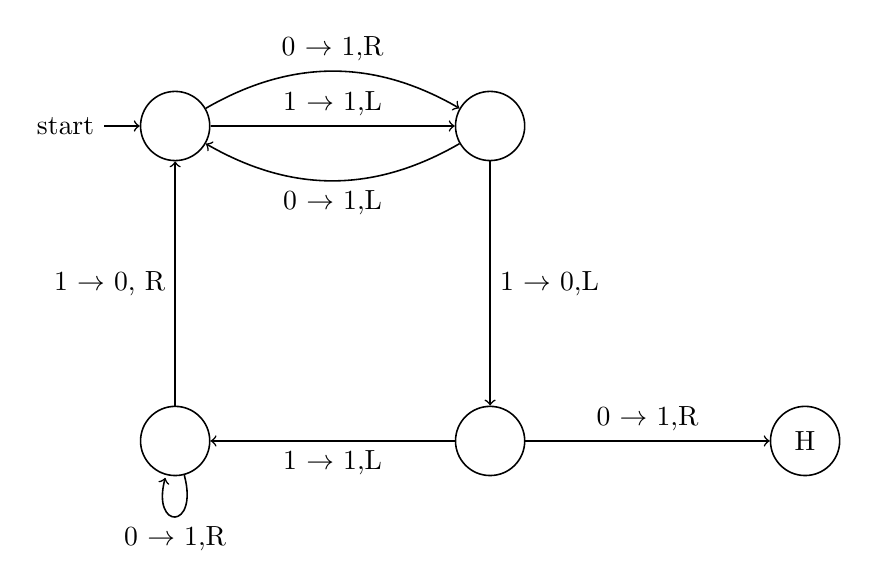
\begin{tikzpicture}[->,auto,node distance=4cm,line width=0.2mm]
  \node[initial,state] (A)              {};
  \node[state] 	(B) [below of=A] {};
  \node[state] 	(C) [right of=A] {};
  \node[state] 	(D) [below of=C] {};
  \node[state]         (E) [right of=D] {H};

  \path (A) edge node   	   {1 $\rightarrow$ 1,L}  (C)
	(A) edge [bend left] node  {0 $\rightarrow$ 1,R}  (C)
	(C) edge [bend left] node  {0 $\rightarrow$ 1,L}  (A)
	(B) edge node 	     {1 $\rightarrow$ 0, R} (A)
	(B) edge [loop below] node {0 $\rightarrow$ 1,R}  (B)
	(D) edge node 	     {1 $\rightarrow$ 1,L}  (B)
	(C) edge node 	     {1 $\rightarrow$ 0,L}  (D)
	(D) edge node	      {0 $\rightarrow$ 1,R}  (E);
\end{tikzpicture}
\end{Verbatim}

\newpage

\section*{Gøyale eksempler}
\begin{itemize}
	\item
	\href{http://www.texample.net/tikz/examples/enderman/}{Enderman}

	\item
	\href{http://www.texample.net/tikz/examples/dartboard/}{Dartboard}

	\item
	\href{http://www.texample.net/tikz/examples/india-map/}{India map}
\end{itemize}

\end{document}